\section{Evaluation}
\label{sec:evaluation}

We apply \sysname on real policies for backbone and data center networks. Our mains goals are to evaluate if its front-end is expressive enough for real-world policies and the time the compiler takes to generate router configurations.

\begin{figure}
  \subcaptionbox{Data center}
    {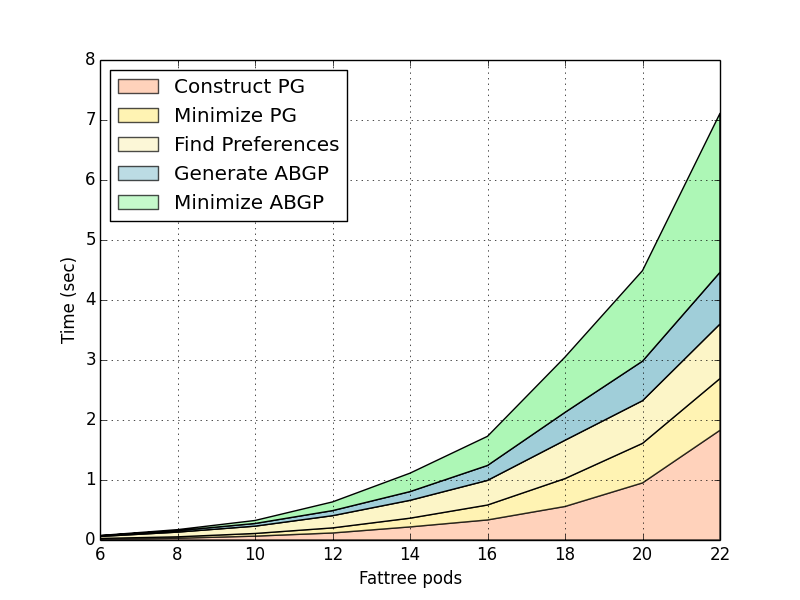
\includegraphics[width=.49\columnwidth]{figures/compilation-times-dc.png}}
  \subcaptionbox{Backbone network}
    {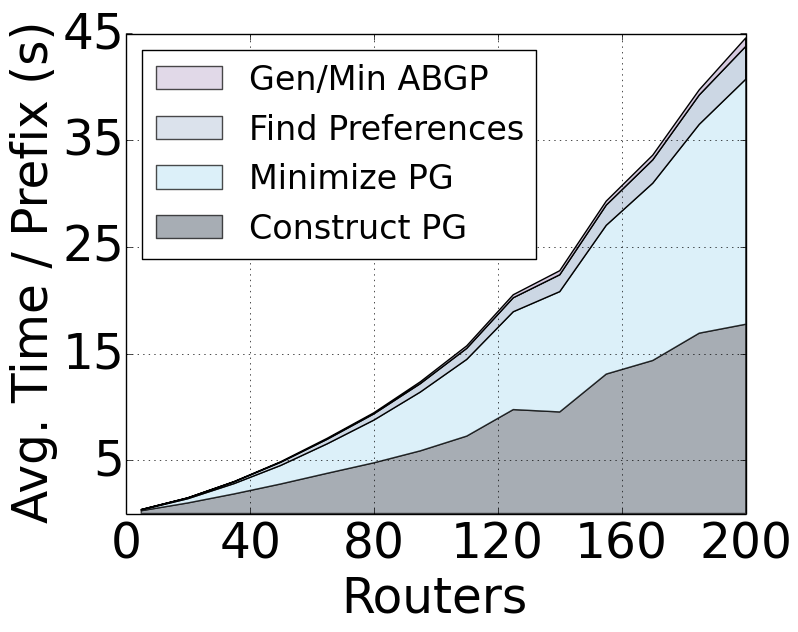
\includegraphics[width=.49\columnwidth]{figures/compilation-times-backbone.png}} \\
  \caption{Compilation time. \label{fig:compilation-times}}
  \vspace{-1em}
\end{figure}


\subsection{Networks studied}

We obtained routing policy for the backbone network and for the data centers of a large cloud provider. Multiple data centers share this policy. The backbone network connects to the data centers and also has many external BGP neighbors. The high-level policies of these networks are captured in an English document which guides operators when writing configuration templates for data center routers or actual configurations for the backbone network (where templates are not used because the network has less regular structure).

The networks have the type of policies that we outline earlier (\S\ref{sec:motivation}). The backbone network classifies external neighbors into several different categories and prefers paths through them in order. It does not want to provide transit among certain types of neighbors. For some neighbors, it prefers some links over the others. It supports communities based on which it will not announce certain routes externally or announce them only within a geographic region (e.g., West Coast of the USA). Finally, it has many filters, e.g., to prevent bogons (private address space) from external neighbors, prevent customers from providing transit to other large networks, prevent traversing providers through peers, etc.

All routers in the datacenter network run BGP using a private AS number and peer with each other and with the backbone network over eBGP. The routers aggregate prefixes when announcing them to the backbone network, they keep some prefixes internal, and attach communities for some other prefixes that should not traverse beyond the geographic region. They also have policies by which some prefixes should not be announced beyond a certain tier in the datacenter hierarchy.

\begin{figure}
  \subcaptionbox{Data center}
    {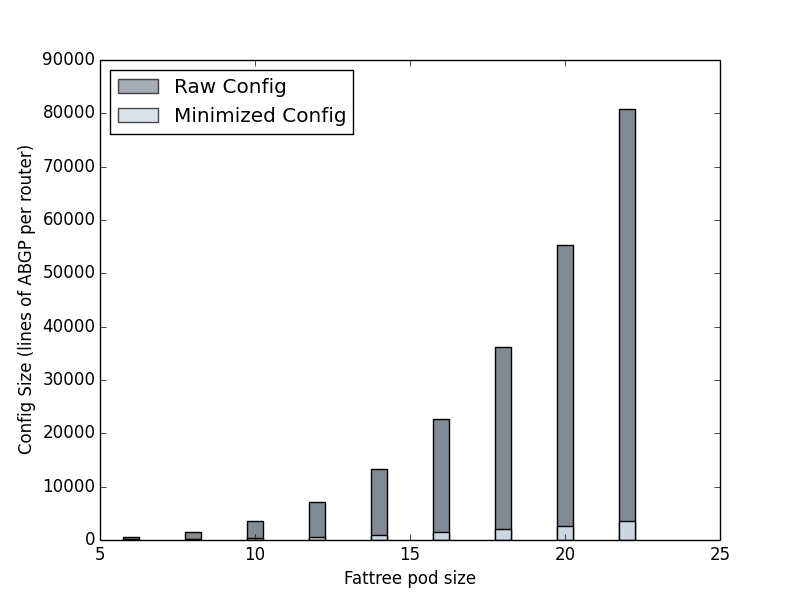
\includegraphics[width=.49\columnwidth]{figures/config-compression-dc.png}}
  \subcaptionbox{Backbone network}
    {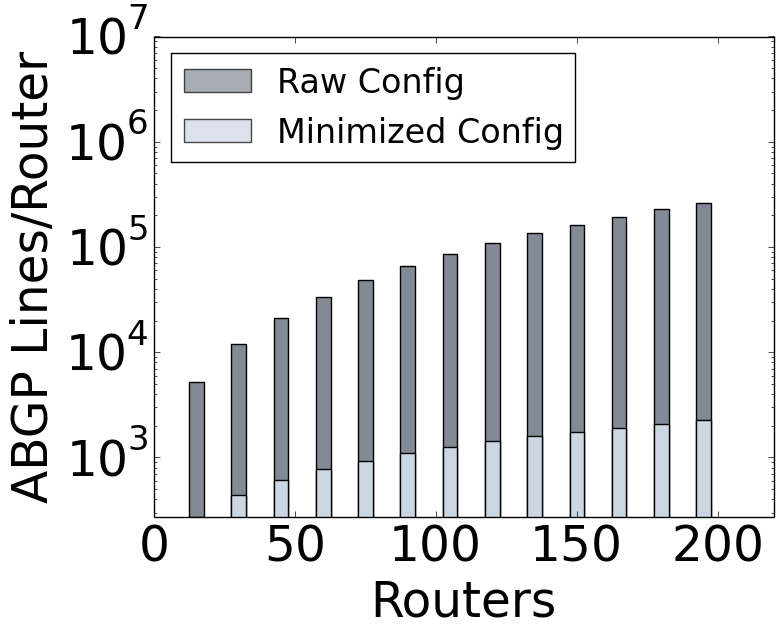
\includegraphics[width=.49\columnwidth]{figures/config-compression-backbone.png}} \\
  \caption{Configuration minimization. \label{fig:config-min}}
  \vspace{-1em}
\end{figure}

\subsection{Expressiveness}

We found that we could translate all network policies to \sysname. We verified with the operators that our translation preserved intended semantics.\footnote{Not intended as a scientific test, but we also asked the two operators if they would find it easy to express their policies in \sysname. The data center operator said that he found the language intuitive. The backbone operator said that formalizing the policy in \sysname seemed equally easy or difficult as formalizing in RPSL~\cite{RFC2622}, but he appreciated that he would have to do it only once for the whole network (not per-router) and did not have to manually compute various local preferences, import-export filters, and MEDs.} We found that the data center policies were correctly translated. For the backbone network, the operator mentioned an additional policy that was not present in the English document, which we added later.

Not counting the lines for various definitions like prefix and customer groups or for prefix ownership constraints, which we cannot reveal because of confidentiality concerns, the \sysname policies were 43 lines for the backbone network and 31 lines for the data center networks.

\subsection{Compilation time}


%\begin{figure}[t!]
%  \centering
%  \begin{minipage}[b]{0.45\linewidth}
%    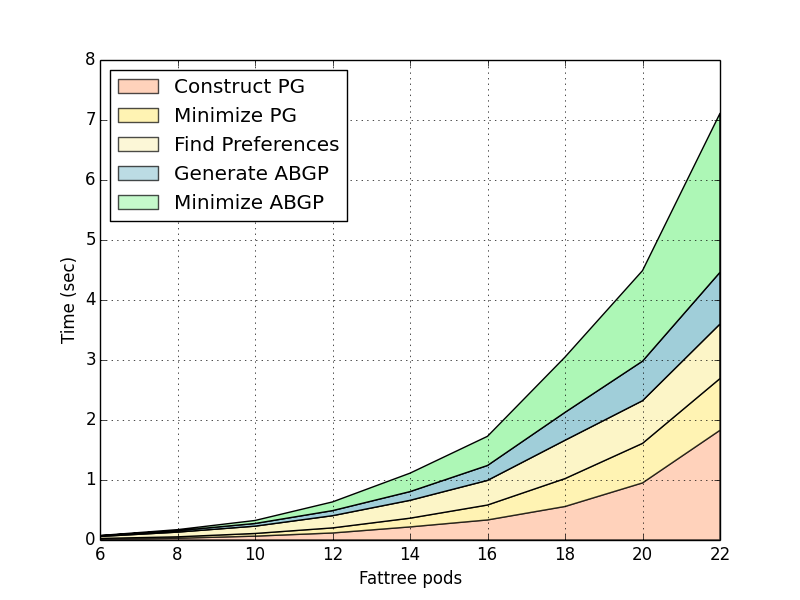
\includegraphics[width=1.1\columnwidth]{figures/compilation-times-dc.png}
%  \end{minipage}
%  \quad
%  \begin{minipage}[b]{0.45\linewidth}
%    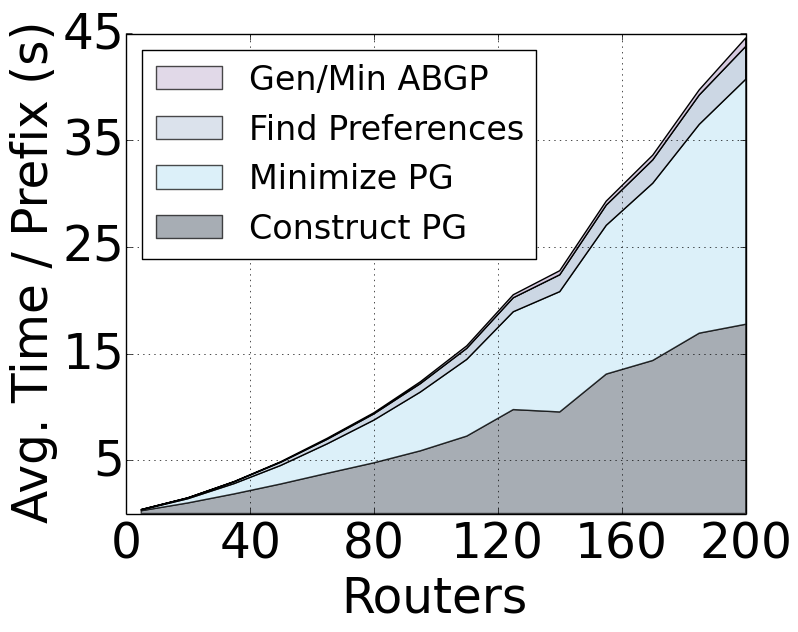
\includegraphics[width=1.1\columnwidth]{figures/compilation-times-backbone.png}
%  \end{minipage}
%  \caption{Compilation times.}
%  \label{fig:compilation-times}
%\end{figure}

%\begin{figure}[t!]
%  \centering
%  \begin{minipage}[b]{0.45\linewidth}
%    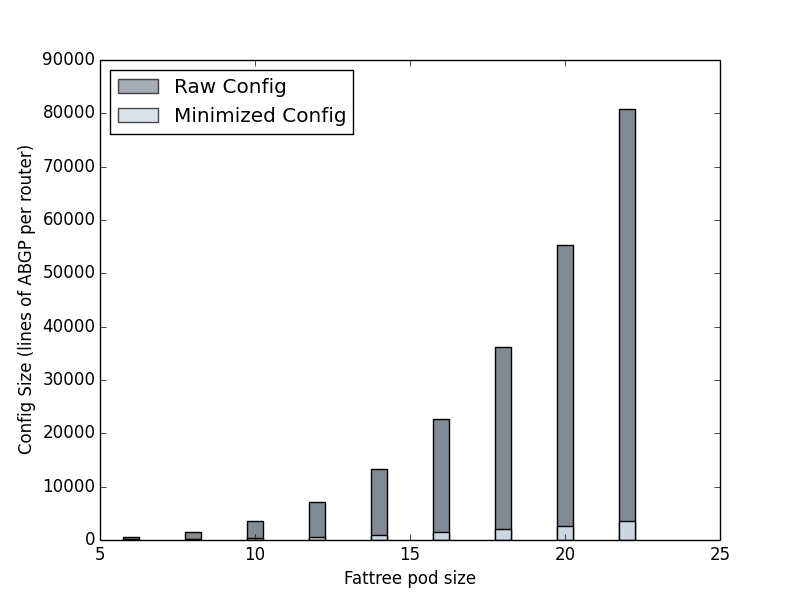
\includegraphics[width=1.1\columnwidth]{figures/config-compression-dc.png}
%  \end{minipage}
%  \quad
%  \begin{minipage}[b]{0.45\linewidth}
%    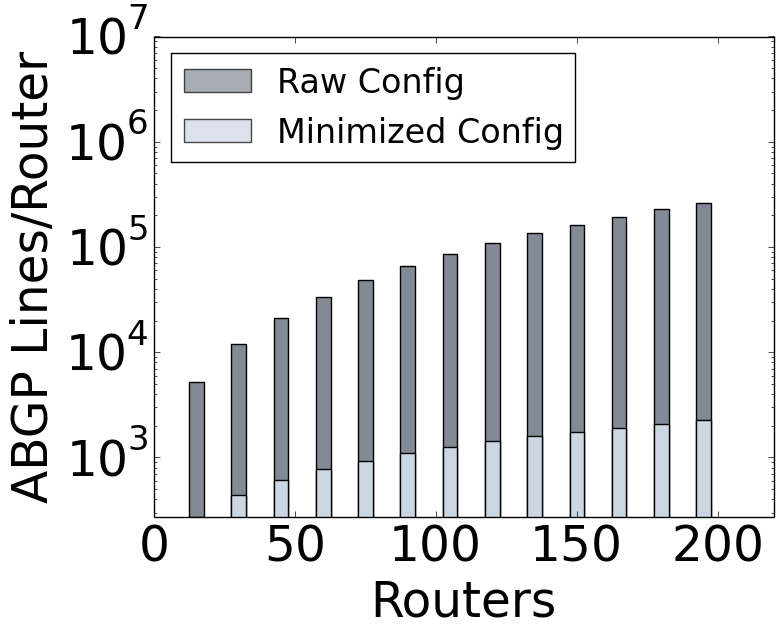
\includegraphics[width=1.1\columnwidth]{figures/config-compression-backbone.png}
%  \end{minipage}
%  \caption{Configuration minimization.}
%  \label{fig:config-minimization}
%\end{figure}

We study the compilation of time for both policies as a function of network size. Even though the networks we study have a fixed topology and size, we can explore the impact of size because our converted policies are network-wide and the compiler takes topology itself as an input. For the data center network, we build and provide as input fat tree~\cite{fattree} topologies of different sizes, assign a /24 prefix to each ToR switch, and randomly map prefixes to each type of prefix group with a distinct routing policy. We take this approach to smoothly explore different sizes. 
%There is a parameterized way to build fat trees~\cite{fattree}, which does not exist for our concrete data center topologies. For a given size, our reported results match those for the concrete topologies.

For the backbone network, the internal topology does not matter since all routers connect in a full iBGP mesh. We explore different mesh sizes and randomly map neighboring networks to routers. Even though each border router connects to many external peers, we count only the mesh size.

All experiments are run on an 8 core, 3.6 GHz Intel Xeon processor running Windows 7.
%
Figure~\ref{fig:compilation-times} shows the compilation times for data centers (a), and backbone networks (b) of different sizes. For both policies, we measure the mean compilation time per prefix since the compiler operates on each prefix in parallel. At their largest sizes, the per-prefix compilation time is roughly 10 seconds for the data center network and 45 seconds for the backbone network.

%From the break down of the time by compilation phase, we see that no single compilation phase dominates the running time of the compiler. However, construction and minimization of the product graph take the most time.

Total compilation for the largest data center is less than 9 minutes total. Unlike the data center policy, the number of prefixes for the backbone policy remains relatively fixed as the topology size increases. Compilation for the largest backbone network, takes less than 3 minutes total. The inclusion of more preferences in the backbone policy increases the size of the PGIR, which leads to PGIR construction and minimization taking proportionally more time.

%


\subsection{Configuration size}

Figure~\ref{fig:config-min} shows the size of the compiled ABGP policies as a function of network size. The naive translation of PGIR to ABGP generates large ABGP policies. To offset this, the compiler performs configuration minimization both both during and after the PGIR to ABGP translation.
%Such minimization is useful for limiting the computational expense of matching routes on BGP routers, reducing the number of forwarding entries in routers in certain cases, and making configurations more readable for humans.
Minimization is highly effective for both the data center and backbone policies. In all cases, minimized policies are a small fraction of the size of their non-minimized counterparts. 

%for i in *.set; do grep bgp $i | wc; done
However, even minimized configurations are hundreds or thousands of lines per router. For the backbone network, the size of \sysname configurations is roughly similar to the BGP components of actual router configurations, though qualitative differences exist (see below). We did not have actual configurations for the data center network; they are dynamically generated from templates. 


\subsection{Propane vs. operator configurations}

Finally, we comment briefly on how \sysname-generated configurations differ from configurations or templates generated by operators.
%
In some cases, \sysname configurations are similar. For example, preferences among neighboring ASes are implemented with a community value to tag incoming routes according to preference, which is then used at other border routers to influence decisions.

In other cases, the \sysname configurations are different, relying on a different BGP mechanism to achieve the same result. Some key differences that we observed were:

$i)$ operators used the no-export community to prevent routes from leaking beyond a certain tier of the datacenter, while \sysname selectively imported the route only below the tier;
%\sysname could use a similar implementation mechanism in the future as an optimization.

$ii)$ operators prevented unneeded propagation of more-specific route announcements from a neighboring AS based on their out-of-band knowledge about the topology, whereas \sysname propagated these advertisements; and

$iii)$ operators used a layer of indirection for community values, using community groups and re-writing values, to implement certain policies in a more maintainable manner, where \sysname uses flat communities.


We are currently investigating if such differences matter to operators (e.g., if they want to read \sysname configurations) and, if necessary, how to reduce them.
